\chapter{Social Engineering}\label{ch:SocialEngineering}

\section{Definitionen des Social Engineering}

Auch zum Thema Social Engineering lassen sich mehrere Definitionen finden, die in vielen Punkten übereinstimmen aber sich auch in wesentlichenn Punkten unterscheiden. 

>>Beim Social Engineering werden menschliche Eigenschaften wie Hilfsbereitschaft, Vertrauen, Angst oder Respekt vor Autorität ausgenutzt, um Personen geschickt zu manipulieren. Cyber-Kriminelle verleiten das Opfer auf diese Weise beispielsweise dazu, vertrauliche Informationen preiszugeben, Sicherheitsfunktionen auszuhebeln, Überweisungen zu tätigen oder Schadsoftware auf dem privaten Gerät oder einem Computer im Firmennetzwerk zu installieren.<<\cite{bsi}

>>Social Engineering benutzt Techniken der Beeinflussung und Überredungskunst zur Manipulation oder zur Vortäuschung falscher Tatsachen, über die sich ein Social Engineer eine gefälschte Identität aneignet. Damit kann der Social Engineer andere zu seinem Vorteil ausbeuten, um mit oder ohne Verwendung von technischen Hilfsmitteln an Informationen zu gelangen.<<\cite{mitn}

In diesen Definitionen wird Social Engineering als etwas rein negatives angesehen das benutzt wird um anderen Personen, zum eigenen Vorteil, zu schaden. In anderen Quellen werden jedoch auch Definitionen dargestellt die aufzeigen dass Sozial Engineering auch zum Vorteil der Zielperson genutzt werden kann.

>>Social Engineering [...] nennt man zwischenmenschliche Beeinflussungen mit dem Ziel, bei Personen bestimmte Verhaltensweisen hervorzurufen, sie zum Beispiel zur Preisgabe von vertraulichen Informationen, zum Kauf eines Produktes oder zur Freigabe von Finanzmitteln zu bewegen.

Gleichzeitig steht Social Engineering für eine Praxis der politischen und gesellschaftlichen Steuerung bzw. Beeinflussung von Gesellschaften mittels Kommunikation und kann sowohl als positiv als auch als negativ wahrgenommene Ergebnisse erzielen. Die stark negative Begriffsvariante dominiert jedoch aktuell das Begriffsbild [...]<<\cite{wiki}

>>Akt der Manipulation einer Person, eine Handlung auszuführen, die vielleicht im besten Interesse der >>Zielperson<< liegt - oder auch nicht.<<\cite{Hadn1}

>>Arzte Psychologen und Therapeuthen nutzen beispielsweise oft Elemente des Social Engineering um ihre Patienten zu bestimmten Handlungen zu manipulieren. Trickbetrüger hingegen nutzen Elemente des Social Engineering um ihre Zielperson zu Aktivitäten zu bringen die zu einem Verlust führen.<< \cite{Hadn1}

Übereinstimmung finden die Definitionen darin, dass es um die Manipulation und oder Beeinflussung von Personen geht um sie zu bestimmten Handlungen zu bewegen   


\section{Geschichte des Social Engineering}

Social Engineering ist ein Phänomen, das es bereits seit Anbeginn der Menschheit gibt, auch wenn es nicht immer unter diesem Begriff bekannt war. Schon kleine Kinder weinen absichtlich, um bei ihren Eltern ihren Willen durchzusetzen, oder nutzen nonverbale Kommunikation, um Dinge zu erreichen, die sie sonst nicht bekämen. Dieses Verhalten zeigt, dass die Manipulation anderer durch gezielte Handlungen tief in der menschlichen Natur verankert ist. (vgl. \cite{SEinNaturdesMenschverankert})

Ein prominentes frühes Beispiel für Social Engineering ist das trojanische Pferd, das als der erste aufgezeichnete Social Engineering Angriff gilt. Diese Episode wurde in Homers "Odyssee" niedergeschrieben. Im Jahr 1184 v. Chr. nutzten die Griechen eine Täuschung, um in Troja einzudringen. Sie bauten ein Holzpferd als Geschenk und täuschten ihren Rückzug vor. Nach der Verkündung dass das Pferd ein Weihegenschenk an die Göttin Athene sei und Unglück bringt sollte es zerstört werden. Außerdem wurde es so groß gebaut damit es nicht in Stadt gebracht werden kann da die Stadt sonst unter dem Schutz der Athene stünde. Die Trojaner holten aufgrund dieser Manipulation das Pferd in die Stadt. Als die Trojaner schliefen, kletterten griechische Soldaten aus dem Holzpferd und öffneten die Tore von innen. (vgl. \cite{troja}).

Zum ersten Mal erwähnt wurde der Begriff Social Engineer in einem Zeitungsartikel der New York Times von 1887. T. Burnett Baldwin wurde darin als Social Engineer bezeichnet, der sichergestellt hat, dass seine Mitarbeiter das Karnevallsprogramm bis ins kleinste Detail ausführten.(vgl. \cite{nytimes1}) Im Jahr 1899 prägte William Tolman den Begriff "Social Engineering" und bezeichnete es als eine der neuesten Professionen. Tolman beschrieb in einem Artikel, wie eine Organisation ein leeres Grundstück in einen Erholungsbereich für die Familien der Mitarbeiter umwandelte, was zu einer verbesserten Beziehung zwischen den Mitarbeitern und dem Arbeitgeber führte.(vgl. \cite{nytimes2}) Dies zeigt, dass Social Engineering darauf zielt, auf eine Personengruppe Einfluss zu nehmen, um ihre Verbindung zu einer bestimmten Organisation zu intensivieren. (vgl. \cite{hist1}).

In der Geschichte der Menschheit finden sich jedoch immer wieder Beispiele dafür, wie Methoden des Social Engineering eingesetzt wurden, um Menschen in eine bestimmte Richtung zu lenken. Durch religiöse Regeln wurden ganze Kulturen geformt, die nach bestimmten Normen und ethischen Grundsätzen handeln, da sie sich davon Vorteile im Jenseits erhoffen. Ein prominentes Beispiel dafür ist das Kastensystem in Indien, das tief in religiösen Überzeugungen und sozialen Strukturen verwurzelt ist und seit Jahrtausenden das Verhalten und die Interaktionen der Menschen bestimmt (vgl. \cite{hindu}).

Ein weiteres Beispiel ist die Verwendung von Propaganda durch politische Regime, um die öffentliche Meinung zu beeinflussen und die Macht zu festigen. Während des Zweiten Weltkriegs nutzten verschiedene Länder intensiv Propaganda, um die Moral zu stärken und die Bevölkerung hinter den Kriegsanstrengungen zu vereinen (vgl. \cite{hisofpropaganda}). Diese gezielte Beeinflussung der Massen zeigt, wie tiefgreifend und wirkungsvoll Social Engineering sein kann.

In modernen Zeiten hat sich Social Engineering weiterentwickelt und ist zu einem zentralen Thema im Bereich der Informationssicherheit geworden. Cyberkriminelle nutzen psychologische Manipulationstechniken, um Menschen dazu zu bringen, vertrauliche Informationen preiszugeben oder schädliche Software herunterzuladen. Dieses Phänomen zeigt, dass Social Engineering nicht nur ein historisches, sondern auch ein aktuelles und sich ständig weiterentwickelndes Thema ist (vgl. \cite{mitn1}).

\section{Grundformen des Sozial Engineering}

Social Engineering in seiner schädlichen Ausprägung lässt sich typischerweise in drei Hauptkategorien einteilen: Phishing, Elizitieren per Telefon und Identitätsbetrug (vgl. \cite{GrundformenDesSE})

\subsection{Phishing}

\begin{figure}[!h]
    \centering
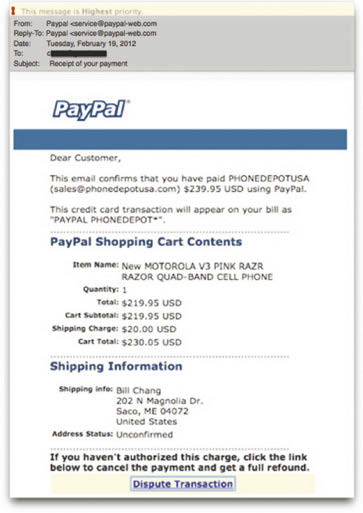
\includegraphics[width = 5cm]{figures/ChristopherHadn_2014_Kapitel2WasIstSocialE_SocialEngineeringEntt.jpg}
\caption{gefälschte E-Mail von PayPal}
\cite{GrundformenDesSE}
\label{fig:PhishingPayPal}
\end{figure}




\subsection{Elizitieren per Telefon}
\subsection{Identitätsbetrug}

\section{Zugangsarten}

\subsection{Elektronisch}
\subsection{Physischer}
\subsection{Soziale Medien}

\section{weitere Angriffsvektoren}

\subsection{Dumpster diving}
\subsection{Watering Hole}
\subsection{Ködern}
\subsection{Honigtopf}
\subsection{Tailgating/Piggybacking}
\subsection{Business Email Compromise}

\section{Psychologische Prinzipien hinter Social Engineering}

\subsection{Mittel der Manipulation}

\subsection{Mittel der Beeinflussung}

\subsubsection{stereotypes Verhalten}
\subsubsection{Reziprozität}
\subsubsection{Verpflichtung und Konsistenz}
\subsubsection{Soziale Bewährtheit}
\subsubsection{Sympathie}
\subsubsection{Authorität}
\subsubsection{Knappheit}

%\section{Beispiel eines erfolgreichen Social Engineering Angriffs}
